	\section{Введение}
	Для уменьшения количества ошибок в программном обеспечении необходимы формальные методы анализа его корректности.
	Многие языки/формализмы можно использовать на этапе спецификации разрабатываемых систем.
	
	
	\section{Системы реального времени}
		Система реального времени (СРВ) — это система, которая должна реагировать на события во внешней по отношению к системе среде или воздействовать на среду в рамках требуемых временных ограничений. 
		Оксфордский словарь английского языка говорит об СРВ как о системе, для которой важно время получения результата. 
		Другими словами, обработка информации системой должна производиться за определённый конечный период времени, чтобы поддерживать постоянное и своевременное взаимодействие со средой.
		
		Под реальным временем понимается количественная характеристика, которая может быть измерена реальными физическими часами, в отличие от логического времени, определяющего лишь качественную характеристику, выражаемую относительным порядком следования событий. 
		
		Для определения рассмотрим три различные аспекта: структурный, функциональный и поведенческий. 
		Функциональный аспект имеет отношение к изменению данных компонентами системы. 
		Поведенческий описывает реакцию системы на внешние воздействия и создавать внутренние события, синхронно или асинхронно.
		Структурный аспект говорит о разбиении системы на модули - подсистемы.
		
		Системы, в которых имеет значение поведенческий аспект называются реактивными. 
		Это системы, которые непрерывно взаимодействуют с окружающим миром.
		Часто реактивные системы многопоточные и распределённые. 
		
		Системы реального времени - подмножество реактивных систем.
		Это такие системы, которые должны удовлетворять явным ограничениям на время ответа.
		Таким системам на этапе создания задаются временные ограничения, благодаря которым, можно определить неполноту или некорректность спецификации и подсистем коммуникации используя формальные методы.
		Главным инструментом для анализа таких ограничений могут быть темпоральные логики.
	\section{От классических логик к темпоральным}
		Основная особенность логической теории состоит в её порядке, который определяет область всех описываемых логикой формул:
		\begin{itemize}
			\item логика высказываний (пропозиционная),
			\item предикатов первого порядка,
			\item предикатов высшего порядка.
		\end{itemize}
		
		Формулы в \textit{логике высказываний} построены на базе пространства элеметарных фактов с использованием множества логических операторов ($ \neg $, $ \wedge $, $ \vee $, $ \Rightarrow $, $ \Leftrightarrow $). 
		Их значения могут быть определены в терминах таблиц истинности или индуктивными правилами по структуре формулы.
		Каждая формула может принимать значения $ true (\top) $ или $ false (\bot) $.
		
		\textit{Логика предикатов первого порядка} (First Order Logic, FOL), добавляет некоторые расширения к логике высказываний:
		\begin{itemize}
			\item Существует пространство элементов, $ D $, на базе которого построены логические формулы;
			\item $ n $-арные $ R_i $ отношения на $ D $ могу быть определены, как подмножество $ D^n $;
			\item $ n $-арный предикат $ p_i $ ассоциирован с каждым отношением $ R_i $.
			Предикат - это функция, которая для каждому элементу $ D_n $ ставит в соответствие значение $ \top $, если он принадлежит $ n $-арному $ R_i $, или $ \bot $ в противном случае.
			\item В ЛППП к операторам логики высказываний добавляются квантор универсальности $ \forall $ (для всех), и квантор существования $ \exists $ (существует).
		\end{itemize}
	Наличие кванторов улучшает выразительность логики, позволяя описывать связи существования и обобщения.
	
	\textit{Логика предикатов высшего порядка} (Higher Order Logic, HOL), расширяет пространство, определённое в ЛППП, позволяя использовать в качестве переменных квантования предикаты. ЛПВП позволяет формально описать логики более низкого порядка.
	
	%\section{Дедуктивная\title{title} система}
	%	Классические логики могут формализовать процесс дедукции: на основе множества утверждений возможно проверить, являются ли другие утверждения следствием первоначального множества.
		
	%	Доказывая теоремы с использованием формальн
	
	\section{Классические логики и время}
	 В общем случае, предположения можно разделить на статические и динамические. 
	 Статические предположения имеют фиксированное и независимое от времени значение истинности, когда значение динамических предположений зависит от времени.
	 Например, утверждение << 1 > 2 >> истинно всегда, но логическое значение утверждения << идёт дождь >> зависит от времени и в некоторые моменты оно может быть верным, а в другие ложным.
	 
	 Т.к. состояние реальных систем изменяется со временем, логические предикаты, описывая их поведение должны предусматривать утверждения, значения которых меняется, в зависимости от времени.
	 Классические логики описывают только атемпоральные формулы, чьи выводимость и разрешимость не зависят от мгновения, в которое они вычисляются.
	 Другими словами, время не играет роли в классической логике; когда утверждение описывает значение, зависимое от времени, время должно быть учтено, как явная переменная. Например, если утверждение $ P $ должно быть верно на интервале $ [t+5,t+20] $, нужно записать формулу, как \[ \forall x \in [t+5,t+20] P(x) \].
	 Такой подход делает описание зависимых от времени утверждений довольно сложным.
	 Для того, чтобы смоделировать поведение в пространствах, в которых логическое значение утверждения может зависеть от времени, созданы модальные и темпоральные логики, как расширение классической логики.
	 Эти подходы облегчают описание отношений во времени.
	 
	\section{Модальная логика}
		В модальной логике концепции правдивости и ложности не статична и неизменна, но относительны и изменчивы.
		В модальных логиках классическая концепция интерпретации формулы расширена так, что каждая модальная логическая теория ассоциирует с формулой не просто одну интерпретацию, а множество интерпретаций, называемых мирами.
		В каждом мире значение истинности связано с формулами также, как в интерпретации формул в классической логике.
		
		Модальная логическая система определяется тройкой $ <W,R,V> $, где $ W $ - множество миров; $ R \subseteq W \times W$ - отношение доступности между мирами; а $ V $ - решающая функция формул: \[ V: F \times W \rightarrow \{\top,\bot\} \], где $ F $ - множество формул модальной теории. $ V $ определена для каждой формулы в $ F $ в каждом мире $ W $.
		
		Формы $ W $ и $ V $ зависят от других характеристик логики; например, является ли она логикой высказываний или ЛППП.
		Кроме операторов и символов классической логики, модальная логика вводит операторы $ \textbf{L} $ (необходимости) и $ \textbf{M} $ (возможности).
		Они описывают концепции необходимости и формул в множестве миров быть доступными в мирах, в которых основная формула вычислена.
		
		Семантика модальной логики может быть формально продемонстрирована с помощью решающей функции, которая индуктивно определена на структуре формулы, которую нужно вычислить. Для модальных операторов $ \textbf{M} $ и $ \textbf{L} $ $ V $ определена следующим образом:
		\begin{itemize}
			\item $ V(\textbf{M}f,w) = \top \Leftrightarrow \exists v \in W. wRv \Rightarrow V(f,v) $;
			\item $ V(\textbf{L}f,w) = \top \Leftrightarrow \forall v \in W. wRv \Rightarrow V(f,v) $
		\end{itemize}
		
		Другими словами, формула $ \textbf{M}f $ истинна в мире $ w $ тогда и только тогда, когда существует мир $ v $, доступный из $ w $, в котором формула $ f $  истинна; формула $ \textbf{L}f $ истинна в мире $ w $ тогда и только тогда, когда во всех мирах, доступных из $ w $,  формула $ f $ истинна.
		Модальные операторы $ \textbf{L} $ и $ \textbf{M} $ имеют простую интерпретацию, как кванторы, определённые на множестве доступных миров из текущего мира: $ \textbf{M} $ - квантор существования, а $ \textbf{L} $ - квантор универсальности. Легко заметить, что между ними присутствует следующая связь: \[ \textbf{L}f = \neg\textbf{M}\neg{f}. \]
		
%		Особенности модальной логики  $ <W,R,V> $ строго связаны с отнощением, определяющим структуру множества миров. 
%		Интерпретаций отношения $ R $ может быть несколько: $ R $ может показывать, как множество классических теорий связаны; например, в немонотонных логиках элементарная истинность и выводимые факты могут изменяться динамически.
%		В контексте темпоральных логик самая интересная интерпретация $ R $ - отношение cktle.o
%	
		
		
	\section{Темпоральные логики}
	 Темпоральные логики - модальные логики, в которых множество миров $ W $ интерпретируется, как множество всех возможных моментов $ T $ временного пространства.
	 
	 Обычно темпоральные логики строятся как расширения классической логики, добавляя множествно новых операторов, скрывающих квантование временного пространства.
	 Темпоральные логики в литературе обычно получаются на основе ЛППП, реже ЛПВП.
	 
	 Как в модальных логиках, где мир, в котором вычисляется формула, указывается явно, в темпоральной логике используется момент времени.
	 Значение формулы - динамическая концепция.
	 Следовательно, концепция разрешимости формулы должна быть изменена так, чтобы она учитывала и интерпретацию формулы и момент времени.
	 
	 В общем темпоральные логики добавляют четыре новых оператора к операторам классической логики \cite{Prior}:
	 \begin{itemize}
	 	\item $ \textbf{G} $ - всегда в будущем;
	 	\item $ \textbf{F} $ - иногда в будущем;
	 	\item $ \textbf{H} $ - всегда в прошлом;
	 	\item $ \textbf{P} $ - иногда в прошлом;
	 \end{itemize}
 
 	Они определяются следующим образом:
 	\begin{itemize}
 		\item $ V(\textbf{G}f,t) = \top \Leftrightarrow \forall s \in T.t<s\Rightarrow V(f,s) $
 		\item $ V(\textbf{H}f,t) = \top \Leftrightarrow \forall s \in T.s<t\Rightarrow V(f,s) $
 		\item $ \textbf{F}f \equiv \neg \textbf{G} \neg f $
 		\item $ \textbf{P}f \equiv \neg \textbf{H} \neg f $
 	\end{itemize}
 	
 	Эти операторы могут выражать концепции необходимости ($ \textbf{G}, \textbf{H} $) и возможности ($ \textbf{F}, \textbf{P} $) в будущем и прошлом соответственно. 
 	Часто в темпоральных логиках эти операторы изображаются другими символами: $ \square $ (всегда) обозначает $ \FutureAlways $, а $ \lozenge $ (иногда) обозначает $ \FutureEventually $.
 	Для операторов прошлого (если они представлены), символ $ \blacksquare $ определяет $ \PastAlways $, а $ \blacklozenge $ - $ \PastEventually $.
 	
 	Если отношение $ < $ предшествования транситивное и нерефлексивное, можно определить два других бинарных оператора:
 	\begin{itemize}
 		\item $ \until $ (или $ \untilShort $): $ \phi_1 \until \phi_2 $ истинно, если $ \phi_2 $ будет истинно в будующем и всё время до этого момента $ \phi_1 $ будет истинно.
 		\item $ \since $ (или $ \sinceShort $) : $ \phi_1 \since \phi_2 $ истинно, если $ \phi_2 $ было истинно в прошлом и всё время с того момента $ \phi_1 $ истинно. 
 	\end{itemize}
 
 	Семантика этих операторов формально определяется так:
 	\begin{itemize}
 		\item $ V(f_1 \until f_2,t) = \true \Leftrightarrow \exists s \in T . t < s \land \forall u \in T . t < u < s \Rightarrow V(f_1,u) $;
 		\item $ V(f_1\since f_2, t) = \true \Leftrightarrow \exists s \in T . s < t \land \forall u \in T. s < u < t \Rightarrow V(f_1,u) $.
 	\end{itemize}
 
 	Заметим, что оператор $ \until(\since) $ не включает текущий момент времени в будущем(прошлом).
 	Введение этих операторов позволяет описать концепции, недоступные с операторами $ \FutureAlways, \PastAlways, \FutureEventually, \PastEventually $.
 	Напротив, последние операторы могут быть определены в терминах $ \until $ и $ \since $.
 	
 	\begin{itemize}
 		\item $ \FutureEventually \phi \equiv \true \until \phi $
 		\item $ \PastEventually \phi \equiv \true \since \phi $
 		\item $ \FutureAlways \phi \equiv \neg \FutureEventually \neg \phi$
 		\item $ \PastAlways \phi \equiv \neg \PastEventually \neg \phi$
 	\end{itemize}
 	
 	Если у темпоральной логики есть свойство начала (т.е. условие, что темпоральное пространство ограничено в прошлом), в операторе $ \since $ нет необходимости.
 	Отношения между событиями могут быть описаны оператором $ \until $, начиная с начального момента времени.
 	
 	Другие распространённые операторы - следования и предшествования, изображаемые символами $ \Next $ и $ \Prev $ соответственно.
 	Эти операторы унарные и могут быть определены в терминах $ \until $ и $ \since $:
 	\begin{itemize}
 		\item $ \Next \phi \equiv \false \until \phi $
 		\item $ \Prev \phi \equiv \false \until \phi $
 	\end{itemize}
 	Эти операторы имеют различные значения в зависимости от структуры времени - например, дискретной или непрерывной - или в случае, если логика основана на событиях.
 	
 	
	\section{Основные характеристики темпоральных логик}
		\subsection{Порядок темпоральной логики}
		 Порядок темпоральной логики - порядок классической логики, на которой основана темпоральная.
		 Эта характеристика описывает множество формул, которые могут быть выражены в данной логике.
		 Более высокий порядок описывает более высокую выразительность, но и более высокую сложность формул, а следовательно, сама логика менее полна и разрешима.\cite{Bucci}
		\subsection{Структура темпорального пространства}
		 Основные свойства модальной логики, а следовательно и темпоральной логики, связаны со свойствами отношения $ R $.
		 Для темпоральных логик отношение $ R $ называется отношением предшествования и обозначается $ < $.
		 Его свойства, влияющие на структуру темпорального пространства:
		 \begin{itemize}
		 	\item \textbf{транзитивность}: $ \forall xyz.x<y \land y<z \Rightarrow x < z  $
		 	\item \textbf{нерефлексивность}: $ \forall x.\neg x < x $
		 	\item \textbf{линейность}: $ \forall xy. x < y \lor x = y \lor y < x$
		 	\item \textbf{линейность слева}: $ \forall xyz. y<x \land z<x \Rightarrow y<z \lor y=z \lor z<y $
		 	\item \textbf{линейность справа}: $ \forall xyz. x<y \land x<z \Rightarrow y<z \lor y=z \lor z<y $
		 	\item \textbf{ограниченность в прошлом}: $ \exists x. \neg y. y<x $
		 	\item \textbf{ограниченность в будущем}: $ \exists x. \neg y. x<y $
		 	\item \textbf{предок}: $ \forall x.\exists y.y<x $
		 	\item \textbf{наследник}: $ \forall x.\exists y.x<y $
		 	\item \textbf{плотность}: $ \forall xy.x<y\Rightarrow \exists z. x<z<y $
		 	\item \textbf{дискретность}: $ ( \forall xy.x<y\Rightarrow \exists z.x<z \land \neg \exists u.x<u<z)\land (\forall xy.x<y\Rightarrow \exists z.z<y \land \neg \exists u.z<u<y) $ 
		 \end{itemize}
	     Обычно отношение $ < $ транзитивно и нерефлексивно.
	     
	     \begin{figure*}[h]
	     	\centering
	     	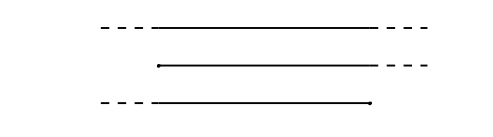
\includegraphics[width=0.7\linewidth]{linear-time}
	     	\caption{Линейные темпоральные пространства}
	     	\label{fig:linear-time}
	     \end{figure*}
		 
		\begin{figure*}[h]
			\centering
			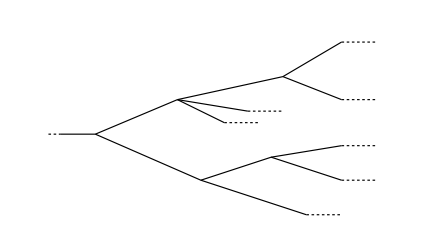
\includegraphics[width=0.7\linewidth]{non-linear-in-future-time}
			\caption{Нелинейное в будущем темпоральное пространство}
			\label{fig:non-linear-in-future-time}
		\end{figure*}
		\subsection{Фундаментальная сущность логики}
		 Простейший способ класификации темпоральных логик - разделение на использующие точки во времени или временные интервалы.
		 Эта характеристика также влияет на выразительность логики.
		 
		 Темпоральные логики основанные на точках описывают отношения между событиями в терминах точек.
		 Интервалы в таких логиках определяются, как связанное множество точек.
		 В таких логиках сложнее описать связи между интервалами, в которых предполагаются некоторые события.
		 Длительность времени выражается с использованием квантования времени.
		 Логики, основанные на временных точках \cite{Manna} \cite{Rosner}, определяют поведение системы на основе некоторых точек во времени; точки определяются особым состоянием системы и при появлении событий, означающих смену состояния.
		 Для описания темпоральных отношений используются операторы $ \futureAlways $ и $ \futureEventually $ для необходимости и возможности соответственно.
		 
		 Темпоральные логики, основанные на интервалах более выразительны, т.к. могут описать события на временных интервалах, а отдельный момент времен представлен единичным интервалом.
		 Обычно интервальные логики запрещают описывать формулы с бОльшим уровнем абстракции, и таким образом более кратки и легки в понимании, чем точечные темпоральные логики.
		 Интервальные логики обычно определяют особые операторы для описания отношения между интервалами, например, как показано на рисунке \ref{fig:interval-relations} для логики Аллена.
		\begin{figure}[h]
			\centering
			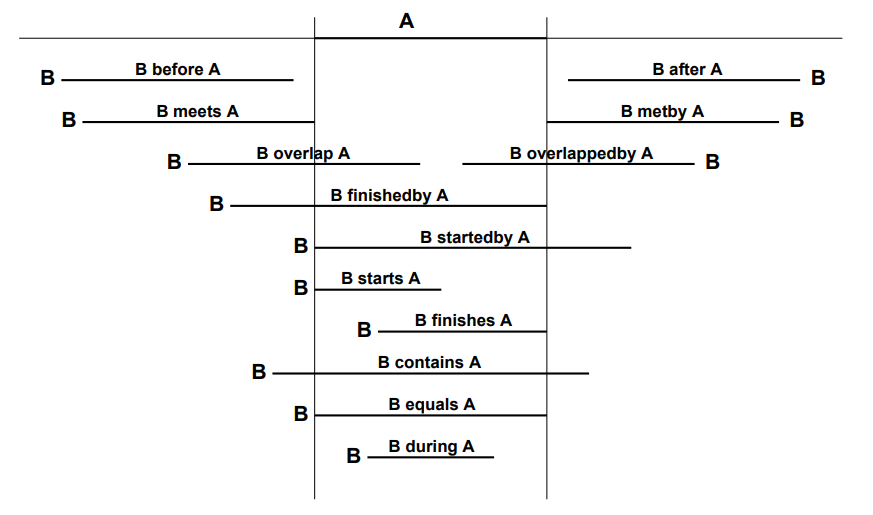
\includegraphics[width=0.7\linewidth]{interval-relations}
			\caption{Возможные отношения между двумя интервалами}
			\label{fig:interval-relations}
		\end{figure}
	
		Отношения между точками или интервалами обычно качественные, однако для определения систем реального времени предпочтительными являются количественные отношения. 
		\subsection{Метрика времени и количественные временные ограничения}
		 Наличие метрики времени определяет возможность выражения темпоральных ограничений в количественной форме в формулах логики; без метрики времени в логике могут присутствовать только только порядковые темпоральные отношения.
		 
		 При наличии метрики времени, становится возможным описание количественных темпоральных отношений, - таких как расстояние между событими, длительность событий, в единицах времени.
		 Описание количественных временных ограничений фундаментально для описания систем реального времени. Типичный способ добавления метрики времени - ввести определение ограниченных операторов, например: \[\futureEventually_{[4,7]}A \]
		 означает, что $ A $ временно истинно на интервале времени от 4 до 7 единиц времени, начиная с текущего момента.
		 Другой способ основан на точном задании системного времени в формулах.
		 
		В определении систем реального времени, основное поведение системы обычно выражается значениями количественных временных ограничений. Правильное поведение системы зависит от разрешимости этих ограничений.
		Можно выделить ограничения на установку связей между появлениями:
		\begin{enumerate}
			\item события и соответствующей реакции (время реакции). Типичное виды:
			\begin{itemize}
				\item максимальное расстояние между событием и реакцией (таймаут);
				\item точное расстояние между событием и реакцией (задержка);
			\end{itemize}
			\item одинаковыми событиями (периодичность). Типичные виды:
			\begin{itemize}
				\item минимальное расстояние между двумя появлениями события.
				\item точное расстояние между появлениями события.
			\end{itemize}
		\end{enumerate}
	
		Такую классификацию можно упростить, уменьшив типы темпоральных ограничений до двух элементарных:
		\begin{itemize}
			\item универсальный темпоральный спецификатор $ \futureAlways_i A $, означающий, что $ A $ верно во все моменты интервала $ i $;
			\item темпоральный спецификатор существования $ \futureEventually_i A $, означающий, что $ A $ верно по крайней мере в один момент времени на интервале $ i $;
		\end{itemize}
		где $ A $ - формула темпоральной логики, а $ i $ - интервал, который может быть как множеством точек, так и фундаментальной сущностью, чьи экстремумы описаны количественно (рис. \ref{fig:temporal-qualificators}).
		
		\begin{figure}[h]
			\centering
			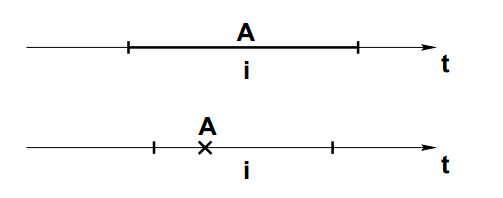
\includegraphics[width=0.7\linewidth]{images/temporal-qualificators}
			\caption{Количественные временные ограничения}
			\label{fig:temporal-qualificators}
		\end{figure}
		
		Используя эти два элементарных оператора можно описать большинство временных требований к системе реального времени:
		\begin{itemize}
			\item после $ A $, должно произойти $ B $ не позднее $ t $ единиц времени: $ A \Rightarrow \futureEventually_{[0,t)}B $
			\item после $ A $, должно произойти $ B $ через $ t $ единиц времени: $ A \Rightarrow \futureEventually_{[t,t]} B $
			\item минимальная задержка между двумя появлениями события $ A $ не меньше $ t $ единиц времени: $ A \Rightarrow \futureAlways_{(0,t)} \neg A $
			\item задержка между двумя появлениями $ A $ должна всегда равняться $ t $ единиц времени: $ A \Rightarrow (\futureAlways_{(0,t)}\neg A) (\futureAlways_{[t,t]}A) $
		\end{itemize}
	
		\subsection{События и очерёдность событий}
		 Типичные причинно-следственные связи могут быть заданы, используя простейшие операторы импликации и эквивалентности. Более того, простейшие операторы ($ \futureAlways, \futureEventually $) темпоральной логики могут быть полезно использованы для описания фактов и правил. Факт - предикат, истинный хотябы раз (т.е. существует событие), а правило - предикат, истинный на протяжение всего времени. Эти операторы, однако, не подходят для описания связей, описывающих последовательность событий, таких как:
		 \begin{enumerate}
		 	\item $ A $ предшествует $ B $;
		 	\item $ A $ следует за $ B $;
		 	\item $ A $ будет истинно, пока $ B $ не станет истинным;
		 	\item $ A $ было истинно с тех пор, огда $ B $ стало истинно в последний раз;
		 \end{enumerate}
	 	где $ A $ и $ B $ - формулы темпоральной логики.
	 	На рисунке \ref{fig:ordering-constraints} приведена иллюстрация данных ограничений, где $ T $ - момент времени, в который происходит вычисление формул.
		\begin{figure*}[h]
			\centering
			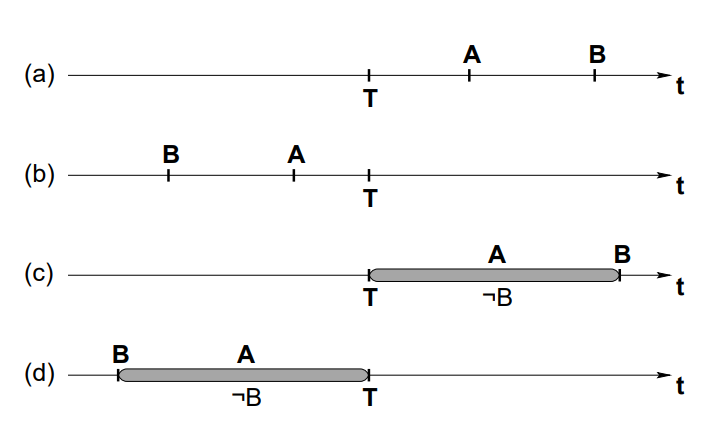
\includegraphics[width=0.7\linewidth]{images/ordering-constraints}
			\caption{Ограничения на порядок следования событий}
			\label{fig:ordering-constraints}
		\end{figure*}
	
		Операции следования в будущем и предшествования в прошлом можно определить, используя операторы $ \until $ и $ \since $:
		\[ A \precede B \equiv \neg((\neg A) \until B) \]
		\[ A \follow B \equiv \neg((\neg A) \since B) \]
		Следовательно, для того, чтобы выразить последовательность между событиями, темпоральная логика должна предоставить операторы $ \until $ и $ \since $
		
		Как следствие, существует множество видов таких операторов. Типичное определение таких операторов - <<слабое>> определение:
		\begin{itemize}
			\item $ A \untilWeak B $ - истинно, когда $ B $ станет истинным и до тех пор, пока $ A $ будет истинным, или если $ B $ всегда ложно, а $ A $ всегда истинно.
			\item $ A \sinceWeak B $ - истинно, когда $ B $ было истинно с того момента, когда $ A $ стало истинным, или если $ B $ всегда было ложно, а $ A $ всегда истинно.
		\end{itemize}
		
		Сильные версии этих операторов предполагают наличие смен состояний для $ B $. То есть они могут быть определены следующим образом:
		\begin{itemize}
			\item $ A \until B \equiv \futureEventually B \land A \untilWeak B $
			\item $ A \since B \equiv \pastEventually B \land A \sinceWeak B $
		\end{itemize}
	
		Также есть и другие версии, в которых текущее время включено в промежутки определения операторов.
		В таком случае так называемая нулевая версия слабых версий операторов определяется так:
		\begin{itemize}
			\item $ A \untilWeakZero B \equiv B \lor (A \land A \untilWeak B)$
			\item $ A \sinceWeakZero B \equiv B \lor (A \land A \sinceWeak B)$
		\end{itemize}
		
		Остальные версии операторов являются комбинациями уже описанных выше вариантов.
		
		\subsection{Время: явное, неявное, абсолютное}
		 Время в темпоральных логиках может быть определено в явном или неявном виде. 
		 Модель времени неявная, когда значения формул зависит от времени, в которое формула вычисляется, и это неявно задаётся в формуле. 
		 Например, $ \futureAlways A $ значит, что:\[\forall t \in [T_0, \infty].A(t) \], где $ T_0 $ - время вычисления формулы (текущий момент времени).
		 Когда время задано неявно, формализм может отражать временной порядок событий.
		 Каждая формула объясняет, что происходит во время её вычисления (например, в прошлом или в будущем),в текущий момент времени:\[\futureEventually \futureEventually_{[3,5]} A \] означает, что $ A $ будет истинно на интервале от 3 до 5 единиц времени в будущем относительно текущего момента времени.
		 Если время рассматривается неявно, возможность сослаться на абсолютное значение времени, на конкретный момент, обычно теряется. 
		 
		 Напротив, когда время задаётся явно, через переменную, возможно описать любое полезное свойство реального времени.
		 Явное задание времени позволяет описать выражение, не имеющее смысла в пространстве времени - например, активацию предиката в момент, когда количественная мера времени нечётна.
		 
		 Ссылка на момент времени может быть абсолютной или относительной.
		 Она считается абсолютной, когда значение времени описывается значением системных часов.
		 Обычно текущее значение системного времени обозначается $ T $; например, в следующей формуле используется абсолютная явная модель времени: \[\forall t.\futureAlways(E \land T = t) \rightarrow \futureEventually (A \land T - t < 10 \text{\emph{ms}}) \], где $ E $ - событие в системе.
		 Когда время представлено в абсолютной форме, значения длительности, дедлайны и таймауты задаются в секундах или миллисекундах.
		 Более того, удовлетворение временным ограничениям зависит от контекста (тип машины, количество процессоров, их загруженность и т.д.).
		 
		 Далее приведена формула, имеющая относительную явную модель времени:\[ \forall t. \futureAlways(E \land T = t) \rightarrow \futureEventually (A \land T - t < 10)\]
		 
		 Чаще всего, время описывается в относительной форме, в единицах времени.
		 В этом случае отношение между этими единицами времени и абсолютным измерением времени, выраженным в секундах (или миллисекундах), не уточняется до фазы реализации системы.
		 Однако, проверка спецификации становится почти независимой от конкретной реализации.
		 
		 \subsection{Логическая разрешимость}
		  Разрешимость темпоральной логики зависит от понятий общезначимости и выполнимости. 
		  Формула выполнима, если существует интерпретация для символов формулы, для который формула верна, тогда как формула называется общезначимой, если она истинна для всех интерпретаций.
		  Темпоральные логики первого порядка (с дискретным временем) не полны, и проблемы выполнимости и общезначимости для них неразрешимы в общем случае.
		  Это в основном обусловлено количественной оценкой зависимых от времени переменных.
		  Запрет таких оценок часто является необходимым условием существования реализуемого механизва автоматической верификации.
		  
		  Выполнимость (общезначимость) является разрешимой проблемой для логики, если существует процедура выявления выполнимости (общезначимости) для каждой формулы логики.
		  Если одна из этих проблем разрешима, доказательство теорем в логике может быть автоматизировано.
		  Это очень важное свойство, т.к. оно увеличивает возможности использования логики, т.к. позволяет создать автоматические средства верификации и валидации описания систем.
		  
		  Существуют и такие логики, семантика которых описана в терминах изменения состояния. 
		  Это делает их приминение более операциональным, чем дескриптивным.
		  Для таких моделей, верификация и валидация часто выполняется с использованием техник проверки модели.
		  К сожалению, для систем реального времени, такая верификация системы во всех её состояниях может быть невыполнима, т.к. будет слишком сложной и занимать очень много времени даже при использовании символьных алгоритмов проверки модели.
		  Семантика, основанная на состоянии, часто ассоциируется с наличием событийной темпоральной логики, или дискретной линейной модели времени.
		  В обоих случаях, определение операционной семантики темпоральной логики очень простое.
		  
		  \subsection{Непротиворечивость и полнота дедуктивной системы}
		   Дедуктивная система - формализация дедуктивного процесса построения доказательства.
		   Дедуктивная система позволяет строить доказательства проще и даёт базу для автоматизации.
		   Эти механизмы часто используются для автоматического и полуавтоматического доказательства теорем.
		   Очевидно, непротиворечивость дедуктивной системы должна быть доказана.
		   
		   Другим желаемым, но не обязательным свойством, является полнота дедуктивной системы; способность строить доказательства для каждой истинной теоремы в логике.
		   Надо отметить, что редко возможно построить полную дедуктивную систему.
		   
	\section{Темпоральные логики для систем реального времени}
		\subsection{Линейная темпоральная логика (пропозиционная)}
			Логика линейного времени (LTL или PTL) введена Пнуэли \cite{PnueliOne}  \cite{PnueliTwo} \cite{PnueliThree}, расширяет логику высказываний, вводя темпоральные операторы $ \futureAlways, \futureEventually, \Next $ и $ \untilShort $. 
			Утверждение в этой логике описывают отношения между состояниями, характеризующими темпоральную эволюцию системы. 
			LTL основана на событиях и не предоставляет метрику для времени.
			
			Системные требования задаются описанием множества ограничений на последовательность событий, которые могут возникнуть в системе, изменяя её состояние.
			Время состоит из последовательность моментов, соответствующих последовательности событий системы.
			В некотором смысле, фундаментальной сущностью логики является момент, в который состояние системы меняется.
			По этим причинам данная логика хорошо совместима с операционными моделями, такими как конечные автоматы.
			
			Темпоральная структура LTL линейна, ограничена в прошлом (существует начальный момент), неограничена в будущем и дискретна (т.е. множество моментов моделируется множеством натуральных чисел). 
			Поэтому представлены только темпоральные операторы будущего. 
			Темпоральные операторы $ \futureAlways, \futureEventually $ и $ \untilShort $ соответствуют операторам $ \FutureAlways, \FutureEventually $ и $ \until $, описаным выше. 
			Формула $ \Next \phi $ является допустимой, если формула $ \phi $ верна в следующих состояниях. 
			Оператор $ \until $ эквивалентен оператору $ \untilWeakZero $, описанному выше. Следовательно, возможно описать требования системы реального времени о последовательности событий в будущем. 
			Асимметрия логики (в связи с ограниченностью в прошлом) и отсутствие оператора $ \since $ не ограничивает спецификацию требований для систем реального времени о последовательности событий в прошлом. 
			Более того, отсутствие метрики времени не позволяет определить любой тип количественных темпоральных ограничений. 
			Следовательно, LTL более приспособлена для использования в реактивных и многопоточных системах, чем в системах реального времени. 
			Реактивные системы обычно событийно-ориентированы и не представляют количественные темпоральные ограничения, такие как таймауты и дедлайны.
			
			
		\subsection{Choppy-логика}
			Choppy-логика, представленная Рознером и Пнуэли \cite{Rosner} - расширение LTL, полученное в результате добавления оператора $ \chop $ (chop).
			Эта логика обладает всеми характеристиками LTL и улучшает её выразительность с помощью оператора $ \chop $, который запрещает связывать последовательности состояний.
			В первом приближении, оператор может рассматриваться, как оператор разделения временных интервалов.
			В частности, последовательность состояний $ \sigma $ является моделью для формулы $ \phi\chop\psi $, если она может быть разделена на две последовательность $ \sigma' $ и $ \sigma'' $ так, что: $ \sigma' $ - модель для $ \phi $, а $ \phi'' $ - модель для $ \psi $.
			Эта логика имеет большую выразительность, хотя требует более сложной процедуры решения.
		
		\subsection{Темпоральная логика ветвящегося времени}
			Темпоральная логика ветвящегося времени (BTTL), введенная Бен-Ари, Пнуэли и Манна \cite{BTTL}, является расширением LTL.
			Её темпоральная структура ветвится в будущем, а следовательно, может быть использована для описания поведения недетерминированных систем.
			Операторы LTL улучшены для взаимодействия с ветвями.
			Определено четыре квантора для следов и состояний на выбраных следах:
			\begin{itemize}
				\item $ \forall \futureAlways $, для всех следов $ \pi $ и всех состояний $ s \in \pi $;
				\item $ \exists \futureAlways $, для хотябы одного следа $ \pi $ и для всех состояний $ s \in \pi $;
				\item $ \forall \futureEventually $, для всех следов $ \pi $ и для хотя бы одного состояния $ s \in \pi $;
				\item $ \exists \futureEventually $, для хотя бы одного следа $ \pi $ и для хотя бы одного состояния $ s \in \pi $.
			\end{itemize}
			
			В некоторых аспектах BTTL практически эквивалентна LTL. Более того, она адаптировала темпоральную структуру ветвления в будущем. 
			Модели формул конечны и могут быть использованы для построения машины конечных состояний, соответствующих формулам.
			Это делает модель операционно-выполнимой.
			Даже с этим улучшением LTL невозможно задать количественные временные ограничения. 
			Следовательно, эта логика также не подходит для описания систем реального времени.
		
		\subsection{Интервальная темпоральная логика}
		 Интервальная темпоральная логика (ITL), описанная Халперном, Манна и Мосзковски \cite{ITL}, а также доработанная в дальнейшем Мосзковски, может считаться расширением LTL. 
		 ITL основана на логике высказываний с темпоральной структурой, ограниченной в прошлом и неограниченной в будущем, дискретной и линейной.
		 Фундаментальная сущность ITL - интервал, созданный из последовательности состояний.
		 Длина интервала определяется количеством состояний в последовательности.
		 ITL не предоставляет метрики времени и относиться к логикам, основанным на событиях.
		 Она применяется для моделирования эволюции цифровых сигналов.
		 ITL расширяет логику высказываний операторами $ \Next $, $ \futureAlways $,$ \futureEventually $ и <<;>> (chop, аналогичный оператору $ \chop $).
		 Семантика всех этих операторов определена в терминах интервалов, а не состояний, как в LTL.
		 Наличие оператора chop делает выводимость формул ITL неразрешимой; хотя, выводимость разрешима для конкретного подкласса формул ITL.
		 
		 В ITL могут быть определены только порядковые характеристики, показывающие качественные отношения событий.
		 Это делает логику менее приспособленной для определения систем реального времени.
		 Для определения характеристик порядка необходимо использовать оператор chop, т.к. в ITL нет оператора $ \until $.
		 Как суррогат метрики времени используется специальный оператор $ \text{Len}(n) $ для расчёта количества состояний в последовательности.
		 Это позволяет задать точную длительность в терминах количества переходов между событиями.
		\subsection{Линейная модальная логика временных интервалов}
			Линейная модальная логика временных интервалов (Propositional Modal Logic of Time Intervals, PMLTI) описана Халперном и Шохэм \cite{PMLTI}.
			Это темпоральная логика, расширяющая LTL.
			Фундаментальная сущность такой логики - интервал, а темпоральные операторы могут описать все возможные отношения между интервалами.
			Темпоральная структура требует только упорядоченности точек интервала. С таким ограничением, структура времени может быть как линейной, так и ветвящейся, ограниченной или неограниченной, непрерывной или дискретной. 
			PMLTI не предоставляет явной метрики времени.
			От выбора конкретной темпоральной структуры зависит сложность решающей процедуры, демонстрирующей общезначимость формул.
			Проблема общезначимости и выполнимости формул могут быть как разрешимы, так и неразрешимы, в зависимости от выбранной темпоральной структуры.
			
			В PMLTI используется метод трансляции темпоральных логических формул в формулы предикатов первого порядка специальной дедуктивной систмы для доказательства теорем.
			Такой подход позволяет применять все подходы  ЛППП.
			
		\subsection{Ветвящаяся темпоральная логика}
		 Ветвящаяся темпоральная логика (Computational Tree Logic, CTL) представлена Кларке, Эмерсоном и Систлой \cite{Clarke} \cite{ClarkeGrumberg}. 
		 Основана на логике высказываний, имеет ветвящуюся структуру времени.
		 Фундаментальная сущность - точка.
		 Добавлены специальные операторы для рассуждения о поведении в терминах некоторых вариантов будущего, называемых последовательностями.
		 Логика очень похожа на BTTL.
		 CTL не предоставляет явной метрики времени.
		 Для верификации спецификации в CTL применяется подход проверки модели, т.к. спецификацию можно смоделировать в виде машины состояний.
		\subsection{Интервальная логика}
		Интервальная логика (Interval Logic, IL) описана Шварцем, Меллиар-Смитом и Вогтом \cite{IL}. 
		Она основана на временных интервалах и логике высказываний.
		Темпоральная структура линейная, ограничена в прошлом и неограничена в будущем.
		IL не представляет явной метрики времени.
		Интервалы ограничены событиями и изменениями состояний системы, описанных формулами.
		То есть, IL - логика, основанная на событиях.
		Типичная формула в IL выглядит следующим образом: \[[\interval]\alpha \], где $ \alpha $ - формула, а $ \interval $ - интервал, который является контекстом, в котором формула $ \alpha  $ общезначима.
		Самая интересная особенность IL - набор инструментов для определения и построения временных интервалов.
		В IL определены ограниченные версии $ \futureAlways, $ и $ \futureEventually $.
		Граница определяется интервалом: $ [\interval]\futureEventually\alpha $ означает, что $ \alpha $ может быть истинно на $ \interval $.
		Границы интервала описываются событиями.
		Из интервала можно выделить начальный и завершающий интервалы.
		Более того, существование интервала с некоторыми характеристиками является событием.
		Наконец, для описания поведения системы, введены операторы \emph{at}, \emph{in} и \emph{after}.
		Они описывают истинность в начале, в течение, или по окончанию интервала соответственно.
		Их можно использовать для построения интервалов.
		Например: $ A \Rightarrow $, как интервал, означает, что интервал начинается, когда начинается интервал A $ A $ и завершается при завершении контекста.
		
		IL позволяет легко описать ограничения на порядок событий, используя инструменты для построения контекста интервалов, но она не позволяет описать количественные временные ограничения.
		
		\subsection{Расширенная интервальная логика}
		Расширенная интервальная логика (Extended Interval Logic, EIL) представлена Меллинар-Смитом \cite{EIL}. 
		Она расширяет IL путём добавления возможности задания некоторых типов количественных временных ограничений.
		Такие расширения позволяют устранить неприменимость IL для систем реального времени в определении типичных ограничений.
		Первое расширение - возможность определить событие на константном временном расстоянии от другого события (положительном или отрицательном): если $ E $ - событие, тогда $ E + 1\text{sec} $ - также событие.
		Второе расширение - возможность ограничения длины интервалов.
		Например: формула $ <2\text{sec} $ истинна, если интервал, на котором она вычисляется имеет длину меньше 2 секунд.
		С помощью этих расширений возможно описать многие ограничения систем реального времени: \[\futureAlways[E\Rightarrow*\text{end}A](<t_e \land * \text{start} A) \] означает, что для каждого появления события $ E $ предикаты $ \text{start} A $ и $ \text{end} A $ (обозначающие интервал, в котором $ A $ истинно) общезначимы на интервале от момента появления $ E $ и до $ E + t_e $.
		В формуле оператор $ * $ означает <<появление>>, а $ \Rightarrow $ означает, что левая граница определяется появлением события $ E $.
		
		\begin{figure*}[h]
			\centering
			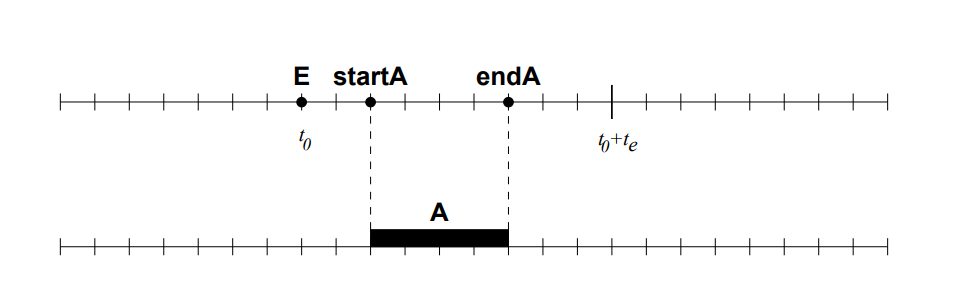
\includegraphics[width=0.7\linewidth]{images/EIL}
			\caption{Графическое изображение примера формулы расширенной интервальной логики}
			\label{fig:eil}
		\end{figure*}
		\subsection{Интервальная логика реального времени}
		Интервальная логика реального времени (Real-Time Interval Logic, RTIL), описанная Разоуком и Горликом \cite{RTIL} - другое расширение IL.
		Её цель - разрешить спецификацию системы реального времени с намерением проверить соответствие между путями выполнения и самой спецификацией системы.
		RTIL вводит метрику времени и даёт возможность присвоить временные значения экстремумам интервалов и строить интервалы, задавая их числовые границы, а не только используя события и смену состояний системы.
		Более того, возможно измерить длительность интервала.
		Эта характеристика делает RTIL интересной для описания систем реального времени. Например, описание, проиллюстрированное на рис. \ref{fig:eil}, можно записать так: \[\futureAlways[\odot E \hookrightarrow t_e] * (\odot \text{start}A \Rightarrow
		 \odot \text{end} A) \]
		 В этом случае, оператор $ * $ означает <<Существует, как подынтервал>>.
		 Специальный оператор $ \odot A$ выделяет момент времени, в которое $ A $ становится истинным. 
		 $ \text{start} A$ и $ \text{end} A $ имеют тот же смысл, что и в EIL.
		 Моменты времени могут быть выражены в абсолютно или относительно начала текущего контекста.
		 RTIL также позволяет задавать количественные ограничения на ограниченном пространстве времени.
		 Эта возможность позволяет сократить написание сложных повторяющихся формул, но не улучшает выразительность логики.
		\subsection{Логика временных интервалов}
		Логика временных интервалов Аллена \cite{Allen} (Logic of Temporal Intervals, LTI) - интервальная темпоральная логика второго порядка.
		В ней интервалы могут разделяться на подынтервалы.
		Интервалы, которые невозможно разбить, являются моментами.
		Темпоральная структура линейна, без дальнейших ограничений.
		Время может быть как дискретным, так и непрерывным.
		LTI не предоставляет метрики времени.
		Темпоральные утверждения описывают отношения порядка между интервалами.
		LTI не полна, но есть способ сделать полное расширение.
		Обе версии, как полная, так и неполная являются разрешимыми.
		Т.к. в LTI невозможно измерить длину интервалов, задание количественных темпоральных ограничений невозможно.
		
		\subsection{Темпоральная логика реального времени}
		Темпоральная логика реального времени (Real-Time Temporal Logic, RTTL) описана Остроффом и Вонхэмом \cite{RTTLWon} \cite{RTTL}. Она расширяет LTL доказательными правилами для свойств реального времени.
		Темпоральная структура линейная и дискретная; фундаментальная сущность - точка.
		Время ограничено в прошлом и неограничено в будущем.
		Время определено и как последовательность состояний, и как последовательность моментов времени.
		Наличие модели, основанной на состояниях, делает RTTL подходящей для подходов проверки модели.
		Таким образом она может служить моделью для валидации маленьких систем.
		Каждый момент времени пронумерован натуральным числом, следовательно, RTTL основана на явной модели времени.
		Существуют системные часы и возможно использовать их в формулах.
		Смена состояний происходит:
		\begin{itemize}
			\item на основе изменения значения часов,
			\item между двумя последовательными моментами времени.
		\end{itemize}
		В случае, когда между двумя последовательными моментами времени появляется больше событий, эти события отличаются только порядком, в котором появляются, но не моментом времени, который с ними ассоциирован.
		Поэтому метрика времени присутствует частично: могут присутствовать неодновременные события, происходящие в один момент времени по системным часам.
		
		Оператор $ \until $ в LTL и оператор $ \until $ в RTTL эквивалентны $ \until_{w0} $. В логике также присутствует оператор $ \Next $. 
		
		\begin{table} [htbp]
			\centering
			\caption{Примеры спецификаций в RTTL}
			\label{table:rttl}%
		\begin{tabular}{|l|l|}
			\hline 
			Значение & RTTL \\
			\hline 
			\hline 
			$ A $ всегда в прошлом & - \\ 
			$ A $ всегда в будущем & $ \Next \futureAlways A $ \\ 
			Всегда $ A $ & - \\
			$ A $ начиная с $ B $ & - \\ 
			$ A $ до $ B $ & $ \Next (A \untilShort B) \lor \futureAlways A $  \\ 
			\hline 
			$ A $ длится до $ t_1 $& $ t= T \rightarrow \futureAlways ((t < T \land T < t + t_1) \rightarrow A) $ \\ 
			$ A $ длилось, начиная с $ t_1 $ & -  \\ 
			$ A $ в пределах $ -t_1 $ в прошлом & - \\ 
			$ A $ в пределах $ t_1 $ в будущем & $ t = T \rightarrow \futureEventually ((t<T \land T<t+t_1) \land A) $  \\ 
			\hline 
			$ A $ в промежутке $ (-t_1, t_2) $& - \\ 
			$ A $ было истинно в $ (-t_1,-t_2) $&-  \\ 
			$ A $ будет истинно в $ (t_1,t_2) $& $ t = T \rightarrow \futureAlways((t+t_1<T\land T<t+t_2)\rightarrow A) $  \\
			$ A $ может быть истинно в $ (t_1,t_2) $& $ t = T \rightarrow \futureEventually((t+t_1<T\land T<t+t_2)\land A) $  \\
			\hline
			$ A $ начиная с $ B $ в течение $ (-t_1, -t_2) $ & - \\  
			$ A $ до тех пор, пока $ B $ в течение $ (t_1,t_2) $ & $ t = T \rightarrow A \untilShort (B\land t+t_1 < T \land T < t+t_2) $ \\ 
			\hline 
		\end{tabular} 
	\end{table}

		<<$ A $ длится до $ t_1 $>> может быть записано в более лаконичной нотации $ \futureEventually_{(0,t_1)}A $, а <<$ A $ до тех пор, пока $ B $ в течение $ (t_1,t_2) $>> может быть задано выражением $ A\untilShort_{(t_1,t_2)} B $. 
		Ситуация, описанная на рис. \ref{fig:eil}, может быть задана варажением: \[\futureAlways(E\rightarrow\Next((\futureEventually_{\leq t_e} \text{end} A) \land \neg (\neg \text{start} A \untilShort \text{end} A)) \]
		
		Для RTTL построена непротиворечивая дедуктивная система, расширяющая дедуктивную систему LTL, но проблема полноты неразрешима.
		
		\subsection{Временная пропозициональная темпоральная логика}
		Временная пропозициональная темпоральная логика (Timed Propositional Temporal Logic, TPTL) - ещё одно расширение LTL, созданное Алуром и Хензингером \cite{TPTL}.
		Как и LTL, TPTL основана на логике высказываний, фундаментальная сущность - момент времени, время линейно, дискретно и ограничено снизу, но неограничено сверху.
		Расширение заключается в добавлении метрики времени: каждый момент соответствует натуральному числу, а монотонная функция ассоциирует значение времени с каждым состоянием системы, делая последовательности состояний представимыми в системе.
		Наличие оператора $ \until $ позволяет задавать порядковые связи.
		Возможность задания числовые темпоральные ограничения - фундаментальная характеристика этой логики.
		Поэтому она подходит для определения систем реального времени.
		В таблице \ref{table:tptl} показаны примеры спецификации в TPTL.
		
			\begin{table} [htbp]
			\centering
			\caption{Примеры спецификаций в TPTL}
			\label{table:tptl}%
			\begin{tabular}{|l|l|}
				\hline 
				Значение & TPTL \\
				\hline 
				\hline 
				$ A $ всегда в прошлом & - \\ 
				$ A $ всегда в будущем & $ \Next \futureAlways A $ \\ 
				Всегда $ A $ & - \\
				$ A $ начиная с $ B $ & - \\ 
				$ A $ до $ B $ & $ \Next ( \untilShort B A) \lor \futureAlways A $  \\ 
				\hline 
				$ A $ длится до $ t_1 $& $ x.\futureAlways y. (x<y<x+t_1) \rightarrow A$ \\ 
				$ A $ длилось, начиная с $ t_1 $ & -  \\ 
				$ A $ в пределах $ -t_1 $ в прошлом & - \\ 
				$ A $ в пределах $ t_1 $ в будущем & $ x.\futureEventually y.(x<y<x+t_1)\land A $  \\ 
				\hline 
				$ A $ в промежутке $ (-t_1, t_2) $& - \\ 
				$ A $ было истинно в $ (-t_1,-t_2) $&-  \\ 
				$ A $ будет истинно в $ (t_1,t_2) $& $ x.\futureAlways y.(x+t_1<y<x+t_2)\rightarrow A $  \\
				$ A $ может быть истинно в $ (t_1,t_2) $& $ x.\futureEventually y.(x+t_1y<x+t_2)\land A $  \\
				\hline
				$ A $ начиная с $ B $ в течение $ (-t_1, -t_2) $ & - \\  
				$ A $ до тех пор, пока $ B $ в течение $ (t_1,t_2) $ & $ x.\Next\untilShort(y.B\land(x+t_1<y<x+t_2))A$ \\ 
				\hline 
			\end{tabular} 
		\end{table}
	
		Ситуация, изображенная на рисунке \ref{fig:eil}, может быть описана формулой: \[\futureAlways x. E\rightarrow(\futureEventually y. \text{end}A\land y \leq x+t_e) \land \neg (\untilShort ~ \text{end}A ~ \neg \text{start} A) \]
		
		Для разрешимости проблемы общезначимости необходимо, чтобы пространство времени было множеством натуральных чисел. 
		Для любого пространства времени с более сложной структурой проблема общезначимости неразрешима.
		Дедуктивная система LTL может быть расширена для TPTL с сохранением полноты и непротиворечивости. 
		Более того, процедура разрешения основана на семантических таблицах и имеется алгоритм проверки модели.
		Это облегчает использование логики для спецификации систем реального времени.
		\subsection{Логика реального времени}
		 Логика реального времени (Ral-Time Logic, RTL), описанная Джаханианом и Моком \cite{RTL}, - это логика, расширяющая ЛППП набором элементов для спецификации систем реального времени.
		 RTL предлагает логический подход для спецификации таких систем, но это не темпоральная логика в классическом её понимании.
		 Она предоставляет абсолютные часы для измерения течения времени.
		 На значение часов можно ссылаться в формулах: Функция <<@>> позволяет присваивать появлению события время.
		 Пространство времени - множество натуральных чисел, линейное, дискретное, ограниченное в прошлом, неограниченное в будущем и линейно упорядоченное.
		 Фундаментальная сущность - момент времени.
		 В RTL возможно указать порядковые и количественные темпоральные ограничения, т.к. возможно задать явно время.
		 Основная проблема RTL - факт того, что существует абсолютное система времени, которое ведёт к очень сложным формулам.
		 Пример, изображенный на рис. \ref{fig:eil} представляется следующим образом:\[\forall t. \forall i. @(\Omega E, i) = t \rightarrow (\exists j.(t<@(\uparrow A,j)) \land (@(\downarrow A, j) \leq t+t_e)) \]
		 Оператор $ \Omega E $ обозначает, что произошло событие $ E $; $ \uparrow A$ -  переключение в значение <<истина>> предиката/сигнала $ A $; $ \downarrow A$ - переключение в значение <<ложь>>; $ i $ и $ j $ - время появления событий, обозначенных оператором $ @ $; $ t $ - время.
		 
		 Дедуктивная система для RTL не представлена, но она кажется реализуемой путём расширения системы ЛППП с законами для новых операторов.
		 
		\subsection{Tempo Reale ImplicitO}
		TRIO - логический язык для спецификации систем реального времени. 
		Название переводится с итальянского, как <<неявное реальное время>>.
		Введен Гхеззи, Мандриоли и Морзенти \cite{TRIO}.
		TRIO расширяет ЛППП специальными предикатами для описания систем реального времени.
		Темпоральная структура линейная и линейно упорядоченная. 
		Возможные пространства времени: натуральные, целые, действительные числа, или интервалы одного из выше указанных типов.
		Фундаментальная темпоральная сущность - точка. 
		Доступна метрика времени.
		Возможно измерить расстояние между двумя точками и длину интервала.
		
		Т.к. TRIO является расширением ЛППП, которое является неразрешимым, следовательно, TRIO также является неразрешимым.
		
		TRIO добавляет два темпоральных оператора:
		\begin{itemize}
			\item $ \Futr{A}{t} $ - $ A $ появляется в момент времени $ t $ в будущем;
			\item $ \Past{A}{t} $ - $ A $ появляется в момент времени $ t $ в прошлом.
		\end{itemize}
		Выше показано, что оба оператора могут быть определены через оператор $ \until $.
		Более того, в TRIO могут быть определены и другие предикаты, как предикаты параметров.
		Это часто позволяется во многих темпоральных логиках, таких как TRIO, MTL.
		Эти операторы позволяют описывать порядковые и количественные ограничения системы, необходимые для определения систем реального времени.
		
		\begin{table} [htbp]
			\centering
			\caption{Примеры спецификаций в TRIO}
			\label{table:trio}%
			\resizebox{\textwidth}{!}{%
			\begin{tabular}{|l|l|}
				\hline 
				Значение & TRIO \\
				\hline 
				\hline 
				$ A $ всегда в прошлом & $ \forall t (t>0 \rightarrow \Past{A}{t}) $- \\ 
				$ A $ всегда в будущем & $ (t>0 \rightarrow \Futr{A}{t})$ \\ 
				Всегда $ A $ & $ \forall t (t>0 \rightarrow \Futr{A}{t}) \land A \land \forall t (t>0 \rightarrow \Past{A}{t}) $\\
				$ A $ начиная с $ B $ & $ \forall t^{``}(t^{``}>0 \rightarrow \Past{A}{t^{``}}) \lor \exists t (t>0 \land \Past{B}{t} \land \forall t^` (0<t^`<t\rightarrow \Past{A}{t}))  $\\ 
				$ A $ до $ B $ & $ \forall t^{``}(t^{``}>0 \rightarrow \Futr{A}{t^{``}}) \lor \exists t (t>0 \land \Futr{B}{t} \land \forall t^` (0<t^`<t\rightarrow \Futr{A}{t}))  $\\ 
				\hline 
				$ A $ длится до $ t_1 $& $ \forall t (0<t<t_1 \rightarrow \Futr{A}{t})$ \\ 
				$ A $ длилось, начиная с $ t_1 $ & $ \forall t (0<t<t_1 \rightarrow \Past{A}{t}) $  \\ 
				$ A $ в пределах $ -t_1 $ в прошлом & $ \exists t (0<t<t_1) \land \Past{A}{t}$ \\ 
				$ A $ в пределах $ t_1 $ в будущем & $ \exists t (0<t<t_1 \land \Futr{A}{t}) $  \\ 
				\hline 
				$ A $ в промежутке $ (-t_1, t_2) $& $ \exists t (0 < t < t_1 \land \Past{A}{t}) \lor A \lor \exists t^` (0<t^`<t_2 \land \Futr{A}{t^`}) $ \\ 
				$ A $ было истинно в $ (-t_1,-t_2) $&$ \Past{\forall t (0<t<t_1-t_2 \rightarrow \Futr{A}{t})}{t_1} $\\ 
				$ A $ будет истинно в $ (t_1,t_2) $& $ \Futr{\forall t (0<t<t_2-t_1 \rightarrow \Futr{A}{t})}{t_1} $  \\
				$ A $ может быть истинно в $ (t_1,t_2) $& $ \Futr{\neg \forall t (0<t<t_2-t_1 \rightarrow \Futr{\neg A}{t})}{t_1}  $  \\
				\hline
				$ A $ начиная с $ B $ в течение $ (-t_1, -t_2) $ & $ \exists t (0<t_2<t<t_1) \land \Past{B}{t} \land \forall t^` (0<t^`<t \rightarrow \Past{A}{t^`})$ \\  
				$ A $ до тех пор, пока $ B $ в течение $ (t_1,t_2) $ & $ \exists t (0<t_2<t<t_1) \land \Futr{B}{t} \land \forall t^` (0<t^`<t \rightarrow \Futr{A}{t^`})$ \\ 
				\hline 
			\end{tabular}}
		\end{table}
	
		Можно ввести дополнительные предикаты, тогда логика будет более лаконичной, однако сложность восприятия вырастет.

		\begin{table} [htbp]
			\centering
			\caption{Примеры спецификаций в расширенной TRIO}
			\label{table:trio-derived}%
			\resizebox{\textwidth}{!}{%
				\begin{tabular}{|l|l|}
					\hline 
					Значение & TRIO \\
					\hline 
					\hline 
					$ A $ всегда в прошлом & $ \AlwP{A} $ \\ 
					$ A $ всегда в будущем & $ \AlwF(A)$ \\ 
					Всегда $ A $ & $ \Alw{A} $\\
					$ A $ начиная с $ B $ & $ \SinceW{B}{A}  $\\ 
					$ A $ до $ B $ & $ \UntilW{B}{A}  $\\ 
					\hline 
					$ A $ длится до $ t_1 $& $ \Lasts{A}{t}$ \\ 
					$ A $ длилось, начиная с$ t_1 $ &$ \Lasted{A}{t} $  \\ 
					$ A $ в пределах $ -t_1 $ в прошлом & $ \WhithinP{A}{t} $ \\ 
					$ A $ в пределах $ t_1 $ в будущем & $ \WhithinF{A}{t}$  \\ 
					\hline 
					$ A $ в промежутке $ (-t_1, t_2) $& $ \Whithin{A}{t_1}{t_2} $ \\ 
					$ A $ было истинно в $ (-t_1,-t_2) $&$ \Past{\Lasts{A}{t_1-t_2}}{t_1} $\\ 
					$ A $ будет истинно в $ (t_1,t_2) $& $ \Futr{\Lasts{A}{t_2-t_1}}{t_1} $  \\
					$ A $ может быть истинно в $ (t_1,t_2) $& $ \Futr{\neg \Lasts{\neg A}{t_2-t_1}}{t_1}  $  \\
					\hline
					$ A $ начиная с $ B $ в течение $ (-t_1, -t_2) $ & $ \SinceB{B}{A}{t_1}{t_2}$ \\  
					$ A $ до тех пор, пока $ B $ в течение $ (t_1,t_2) $ & $ \UntilB{B}{A}{t_1}{t_2}$ \\ 
					\hline 
			\end{tabular}}
		\end{table}
	
	 \FloatBarrier
		Описанную на рис. \ref{fig:eil} задачу можно записать следующим образом: \[ \Alw{E \rightarrow \exists t ((0 < t < t_e) \land \Futr{\text{end} A}{t}\land \WhithinF{\text{start}A}{t})} \]
	
		Для TRIO существует дедуктивная система.
		Она используется в основном для валидации и верификации системных требований через тестирование активности.
		
		\subsection{Метрическая темпоральная логика}
		Метрическая темпоральная логика (Metric Temporal Logic, MTL) описана Коймансом \cite{MTL}. 
		Она расширяет ЛППП темпоральными операторами модальной логики: $ \FutureAlways, \FutureEventually, \PastAlways, \PastEventually $.
		MTL включает метрику времени при выполнений некоторых условий над темпоральным пространством.
		Одно из таких условий - линейная упорядоченность.
		Таким образом, необходима линейная структура.
		
		Фундаментальная сущность логики - точка во времени.
		
		\begin{table} [htbp]
			\centering
			\caption{Примеры спецификаций в MTL}
			\label{table:mtl}%
			\resizebox{\textwidth}{!}{%
				\begin{tabular}{|l|l|}
					\hline 
					Значение & MTL \\
					\hline 
					\hline 
					$ A $ всегда в прошлом & $ \PastAlways A $ \\ 
					$ A $ всегда в будущем & $ \FutureAlways A$ \\ 
					Всегда $ A $ & $ \PastAlways A \land A \land \FutureAlways A $\\
					$ A $ начиная с $ B $ & $ \PastAlways A \lor \exists t (t>0 \land  \PastEventually_t B \land \PastAlways_{<t}A) $\\ 
					$ A $ до $ B $ & $ \FutureAlways A \lor \exists t (t>0 \land  \FutureEventually_t B \land \FutureAlways_{<t}A)  $\\ 
					\hline 
					$ A $ длится до $ t_1 $& $ \FutureAlways_{<t_1}A$ \\ 
					$ A $ длилось, начиная с$ t_1 $ &$ \PastAlways_{<t_1}A$  \\ 
					$ A $ в пределах $ -t_1 $ в прошлом & $ \PastEventually_{<t_1}A $ \\ 
					$ A $ в пределах $ t_1 $ в будущем & $ \FutureEventually_{<t_1}A$  \\ 
					\hline 
					$ A $ в промежутке $ (-t_1, t_2) $& $ \PastEventually_{<t_1} A \land A \land \FutureAlways_{<t_2} A $ \\ 
					$ A $ было истинно в $ (-t_1,-t_2) $&$ \PastEventually_{t_1} ( \PastAlways_{<(t_1-t_2)A}) $\\ 
					$ A $ будет истинно в $ (t_1,t_2) $& $ \FutureEventually_{t_1} ( \FutureAlways_{<(t_2-t_1)A})  $  \\
					$ A $ может быть истинно в $ (t_1,t_2) $& $ \FutureAlways_{t_1} ( \FutureEventually_{<(t_2-t_1)A})  $  \\
					\hline
					$ A $ начиная с $ B $ в течение $ (-t_1, -t_2) $ & $ \exists t (t_2 < t < t_1 \land \PastEventually_{t}B \land \PastAlways_{<t}A)$ \\  
					$ A $ до тех пор, пока $ B $ в течение $ (t_1,t_2) $ & $ \exists t (t_1 < t < t_2 \land \FutureEventually_{t}B \land \FutureAlways_{<t}A) $ \\ 
					\hline 
			\end{tabular}}
		\end{table}
		\FloatBarrier
		Пример с рисунка \ref{fig:eil} может быть описан в MTL: \[E\rightarrow \exists t(0<t<t_e \land \FutureEventually_t \text{end}A\land \FutureEventually_{<t} \text{start}A) \]
		MTL неразрешима, но существует дедуктивная система.
		\subsection{Логика временных интервалов с операторами композиции}
		Логика временных интервалов с операторами композиции (Time Interval Logic with Compositional Operators, TILCO) описана Маттолини и Неси \cite{TILCO} и является темпоральной логикой для описания систем реального времени.
		TILCO расширяет ЛППП и использует интервал как фундаментальную сущность даже если интервал определён через другие интервалы времени.
		Темпоральная структура линейна и предоставляет метрику времени, ассоциирующую целое число каждому моменту времени. 
		Явно указывать временные ограничения кванторам нельзя.
		
		В TILCO один и тот же формализм используется и для спецификации системы, и для описания высокоуровневых условий, которым должна удовлетворять система.
		Они должны быть проверены на этапе валидации системы.
		
		Базовые темпоральные операторы TILCO - кванторы существования и общности ($ @ $ и $ ? $ соответственно), и операторы $ \until $ и $ \since $.
		Эти операторы позволяют кратко описать темпоральные требования, отношения порядка появления и числовые расстояния между событиями; таким образом TILCO полностью поддерживает спецификацию систем реального времени.
		
		TILCO также характеризуется своими операторами композиции, работающими с интервалами: $ , $ соотвествует $ \land $, $ ; $ соответствует $ \lor $ для интервалов.
		Операторы композиции предполагают разную логику при использованием с кванторами существования и общности:
		\begin{itemize}
			\item $ A @ i,j \equiv (A@i)\land(A@j) $,
			\item $ A?i,j \equiv (A?i)\land(A?j) $,
			\item $ A@i;j \equiv (A@i) \lor (A@j) $,
			\item $ A?i;j \equiv (A?i) \lor (A?j) $.
		\end{itemize}
		Другие интервальные операторы пересечения $ \cap $ и объединения $ \cup $ определены путём рассматривания интервалов, как множеств.
		
		\begin{table} [htbp]
			\centering
			\caption{Примеры спецификаций в TILCO}
			\label{table:tilco}%
			\resizebox{\textwidth}{!}{%
				\begin{tabular}{|l|l|}
					\hline 
					Значение & TILCO \\
					\hline 
					\hline 
					$ A $ всегда в прошлом & $ A@(-\infty,0) $ \\ 
					$ A $ всегда в будущем & $ A@(0,\infty)$ \\ 
					Всегда $ A $ & $ A@(-\infty,\infty) $\\
					$ A $ начиная с $ B $ & $\since(B,A)$\\ 
					$ A $ до $ B $ & $ \until(B,A) $\\ 
					\hline 
					$ A $ длится до $ t_1 $& $ A@(0,t_1)$ \\ 
					$ A $ длилось, начиная с$ t_1 $ &$ A@(-t_1,0)$  \\ 
					$ A $ в пределах $ -t_1 $ в прошлом & $ A@(-t_1,0)$ \\ 
					$ A $ в пределах $ t_1 $ в будущем & $ A?(0,t_1)$  \\ 
					\hline 
					$ A $ в промежутке $ (-t_1, t_2) $& $ A?(-t_1,t_2)$ \\ 
					$ A $ было истинно в $ (-t_1,-t_2) $&$ A@(-t_1,-t_2) $\\ 
					$ A $ будет истинно в $ (t_1,t_2) $& $ A@(t_1,t_2) $  \\
					$ A $ может быть истинно в $ (t_1,t_2) $& $ A?(t_1,t_2)  $  \\
					\hline
					$ A $ начиная с $ B $ в течение $ (-t_1, -t_2) $ & $ B?(-t_1,-t_2) \land \since(B,A) @ [-t_2,-t_2] \land A@[-t_2,0) $ \\  
					$ A $ до тех пор, пока $ B $ в течение $ (t_1,t_2) $ & $ B?(t_1,t_2) \land \until(B,A) @ [t_1,t_1] \land A@(0,t_1]  $ \\ 
					\hline 
			\end{tabular}}
		\end{table}
		
	    Опишем пример из \ref{fig:eil} в TILCO: \[E\rightarrow \text{end} A ? (0,t_e] \land \neg \until (\text{end} A, \neg \text{start} A) \]
		
		Для TILCO существует непротиворечивая дедуктивная система.
		TILCO неразрешима, т.к. расширяет ЛППП, однако, она разрешима, если использовать только ограниченные множетсва в качестве ограничений кванторов.
	\section{Вывод}
		
		Таблица \ref{table:discussion} иллюстрирует характеристики рассмотренных темпоральных логик.
		
		\begin{table} [htbp]
			\centering
			\caption{Сравнение представленных темпоральных логик}
			\label{table:discussion}%
			\resizebox{\textwidth}{!}{%
				\begin{tabular}{|l|l|l|c|c|c|c|c|c|}
				\hline
				Логика & Порядок & \multiline{Фундаментальная\\сущность}  & \multiline{Темпоральная\\структура} & Метрика & Разрешимость & \multiline{Дедуктивная\\система} & \multiline{Явная,\\Неявная}\\		
				\hline
				LTL & ЛВ & Точка & Линейная & Нет & Да & Да & Неявная\\	\hline
				Choppy & ЛВ & Точка & Линейная & Нет & Да & Да & Неявная\\ \hline
				BTTL & ЛВ & Точка & Ветвящаяся & Нет & Да & Да & Неявная\\ \hline	
				ITL & ЛВ & Интервал & Линейная & Нет & Да & Да & Неявная\\ \hline
				PMLTI & ЛВ & Интервал & \multiline{Линейная/\\Ветвящаяся} & Нет & Да & Неизвестна & Неявная\\\hline
				CTL & ЛВ & Точка & Ветвящаяся & Нет & Да & Неизвестна & Неявная\\\hline
				IL & ЛВ & Интервал & Линейная & Нет & Да & Неизвестна & Неявная\\\hline
				EIL & ЛВ & Интервал & Линейная & Да & Да & Неизвестна & Неявная\\\hline
				RTIL & ЛВ & Интервал & Линейная & Да & Да & Неизвестна & Неявная\\\hline
				LTI & ЛПВП & Интервал & Линейная & Нет & Да & Да & Неявная\\\hline
				RTTL & ЛППП & Точка & Линейная & Да & Нет & Да  & Явная\\\hline
				TPTL & ЛВ & Точка & Линейная & Да & Да & Да  & Явная\\\hline
				RTL & ЛППП & Интервал & Линейная & Да & Нет & Неизвестна & Неявная\\\hline
				TRIO & ЛППП & Точка & Линейная & Да & Нет & Да  & Неявная\\\hline
				MTL & ЛППП & Точка & Линейная & Да & Нет & Да & Неявная\\\hline
				TILCO & ЛППП & Интервал & Линейная & Да & Да & Да & Неявная\\\hline
			\end{tabular}
			}
		\end{table}
	
		Описанные логики можно разделить на две категории: логики без метрики времени и с ней.
		Логики первой категории меньше подходят для спецификации систем реального времени, т.к. они не поддерживают числовые темпоральные ограничения.
		
		Важным фактором также является возможность использования методов верификации.
		Эта возможность зависит от разрешимости логики. Таким образом логики EIL, RTIL, TPTL и TILCO более предпочтительны среди прочих.
		
		Логики, основанные на ЛППП позволяют описывать спецификацию на более высоком уровне абстракции.
		
		Исходя из выше сказанного, TILCO представляется наиболее подходящей логикой для описания систем реального времени.